\part*{Appendix}
\addcontentsline{toc}{chapter}{Appendix}
\renewcommand{\thesection}{\arabic{section}}
\renewcommand{\theequation}{\arabic{equation}}
\section{Appendix One: Consumer Application}\label{section:Appendix One: Consumer Application}

Another task for the Interdisciplinary Project was to create a consumer application. The aim of the application is to give the person who just ordered information about the delivery. This includes the current step in the delivery process as well as the current position of the driver on a map. After the process the customer should be able to rate the delivery.\newline
The moment the customer finishes placing an order the backend should create an account for the customer. The credentials for the new user should be send to the customer by email. The email also directs to the application in the Play Store where it can be downloaded. This part has to be implemented in the backend if it should be used in a real scenario.\newline
The user can login into the application (Fig. \ref{fig:consumer_application}, left) by entering the user data. Right now a driver account is used to demonstrate the functionality since the backend does not support the right manage to let users see orders owned by drivers.\newline
When the customer enters the application the screen in the middle of Figure \ref{fig:consumer_application} is shown. In this screen \texttt{assigning\_to\_driver} is shown as status. This means the driver cannot be tracked yet since the order has not been assigned to a driver. The application queries every 10 seconds for a status change on the server. As soon as the driver has accepted the order the status switches to \texttt{pickup\_started} (Figure \ref{fig:consumer_application}, right). From now on the position of the driver is updated every 10 seconds so the customer using the application always sees where his delivery is at the moment.
\begin{figure}[htp]

\centering
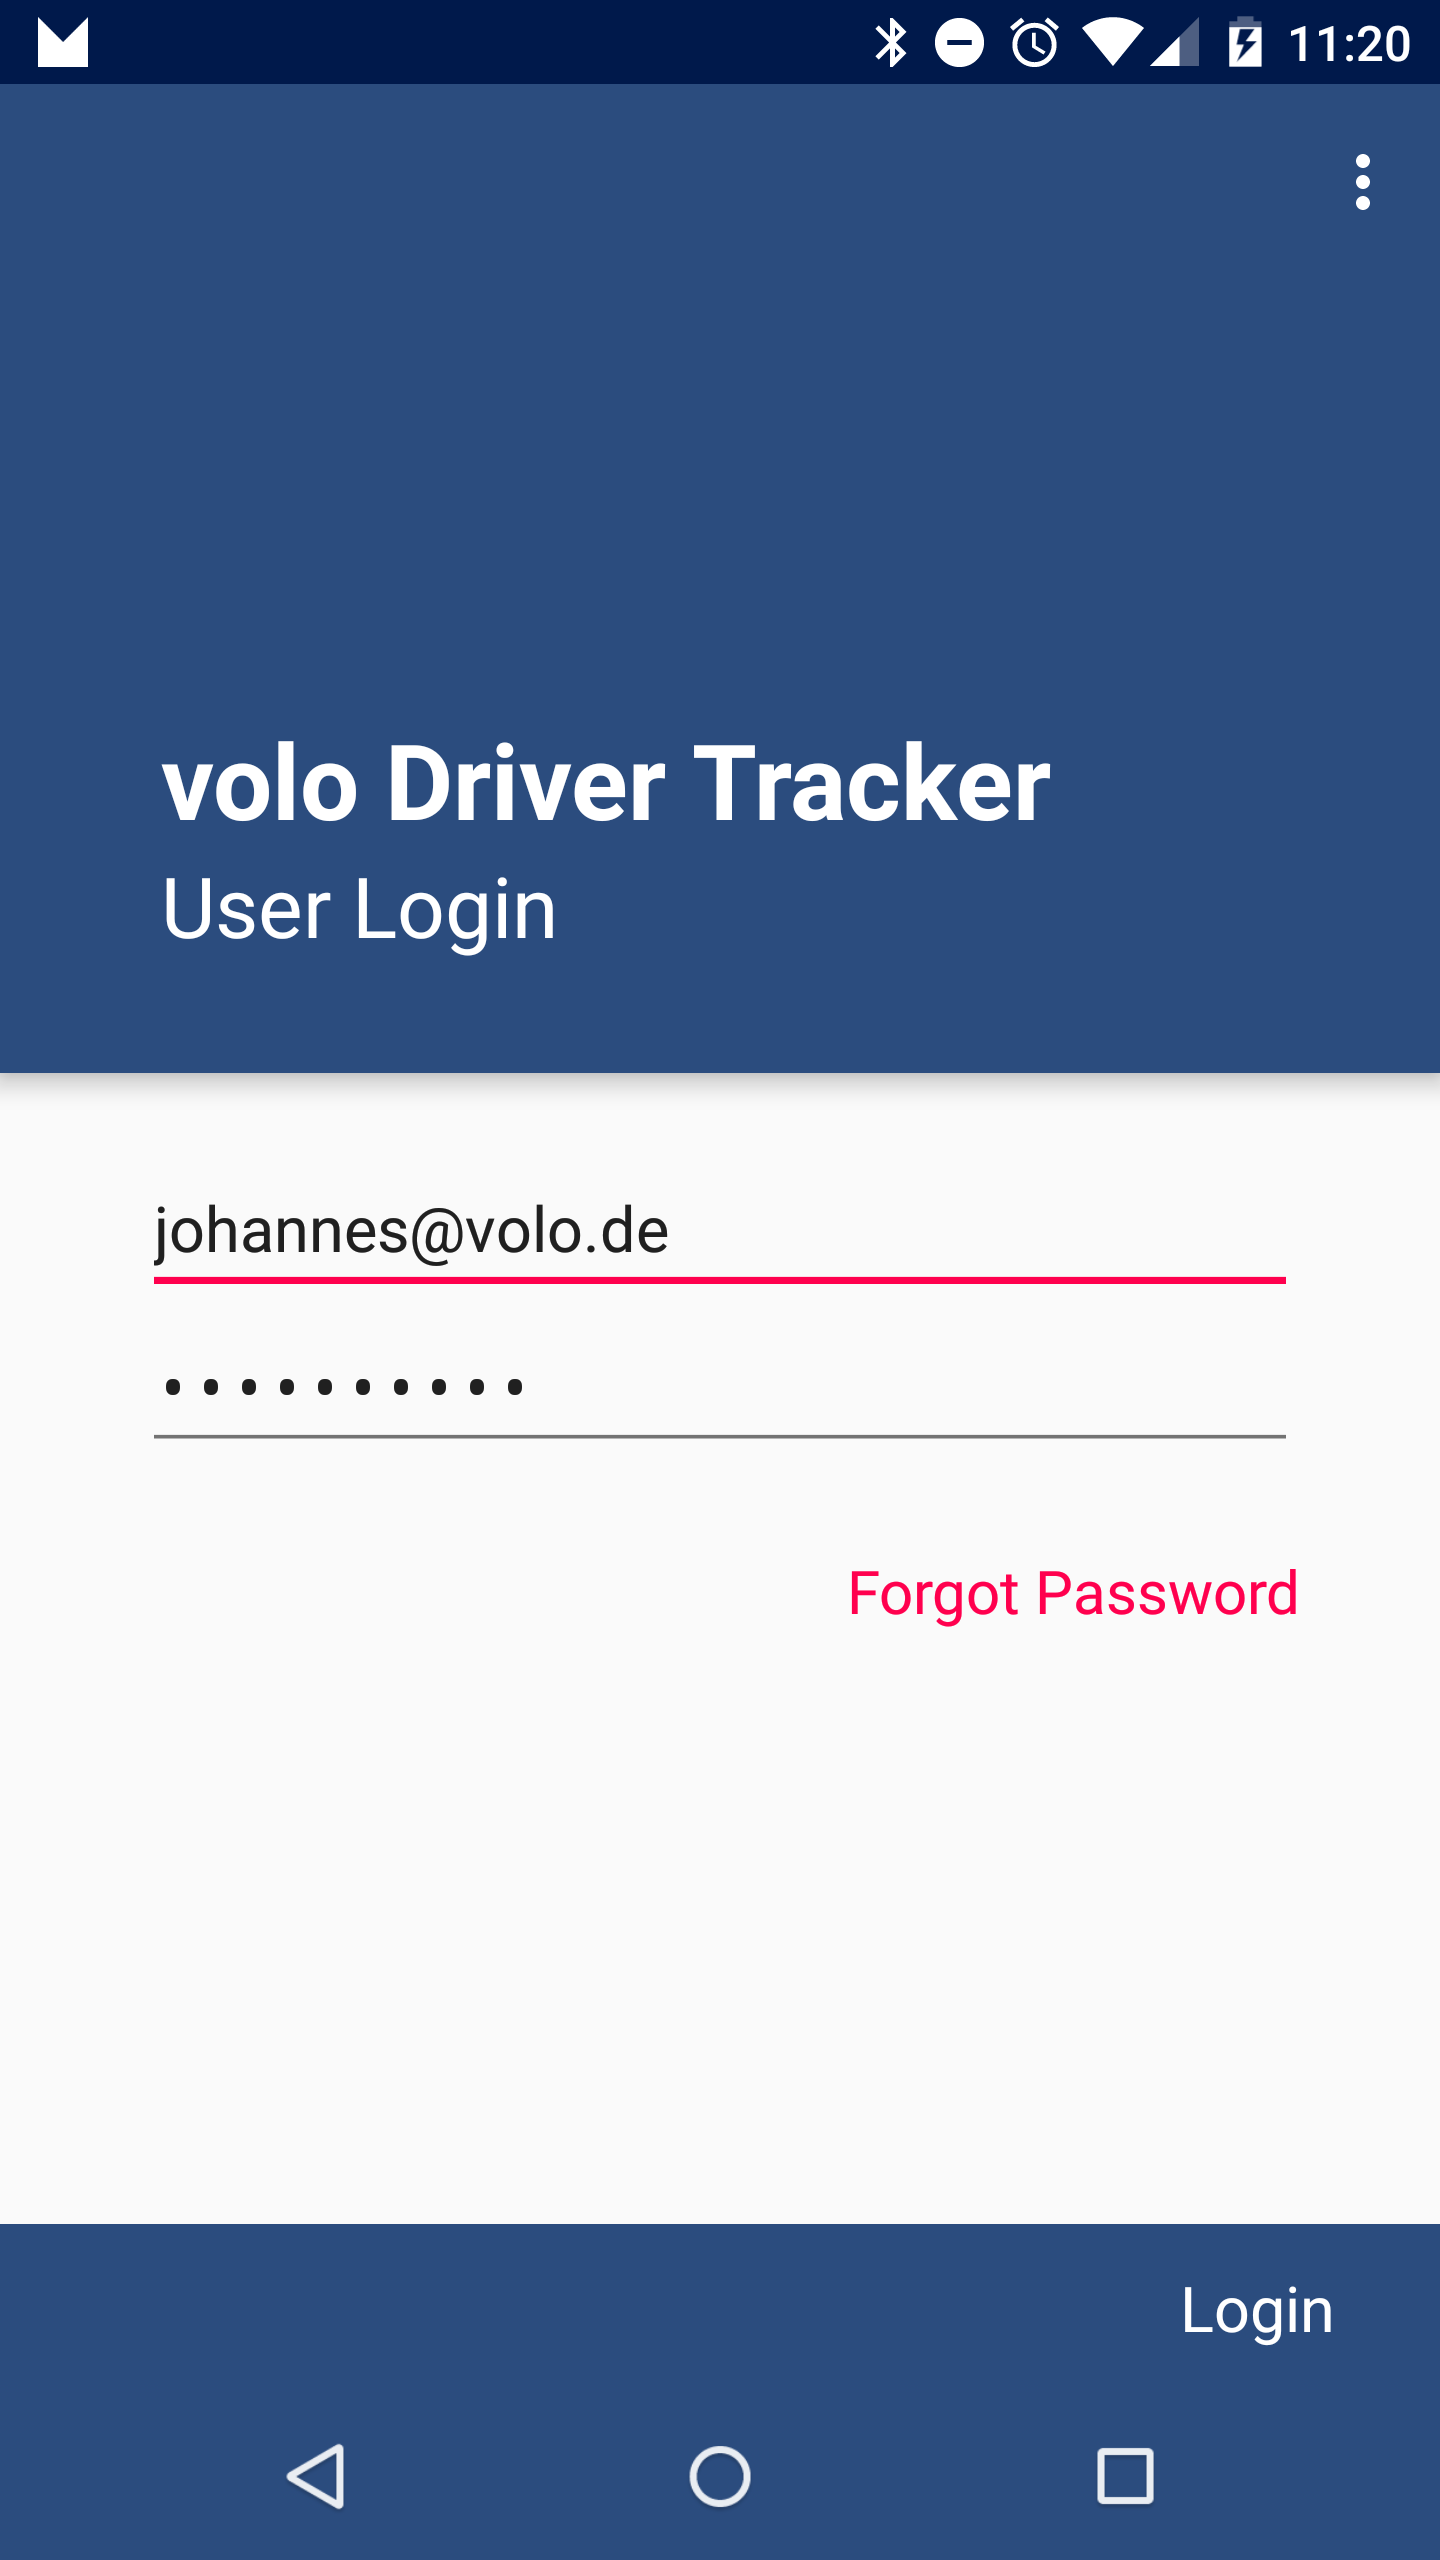
\includegraphics[width=.3\textwidth]{images/1_login.png}\hfill
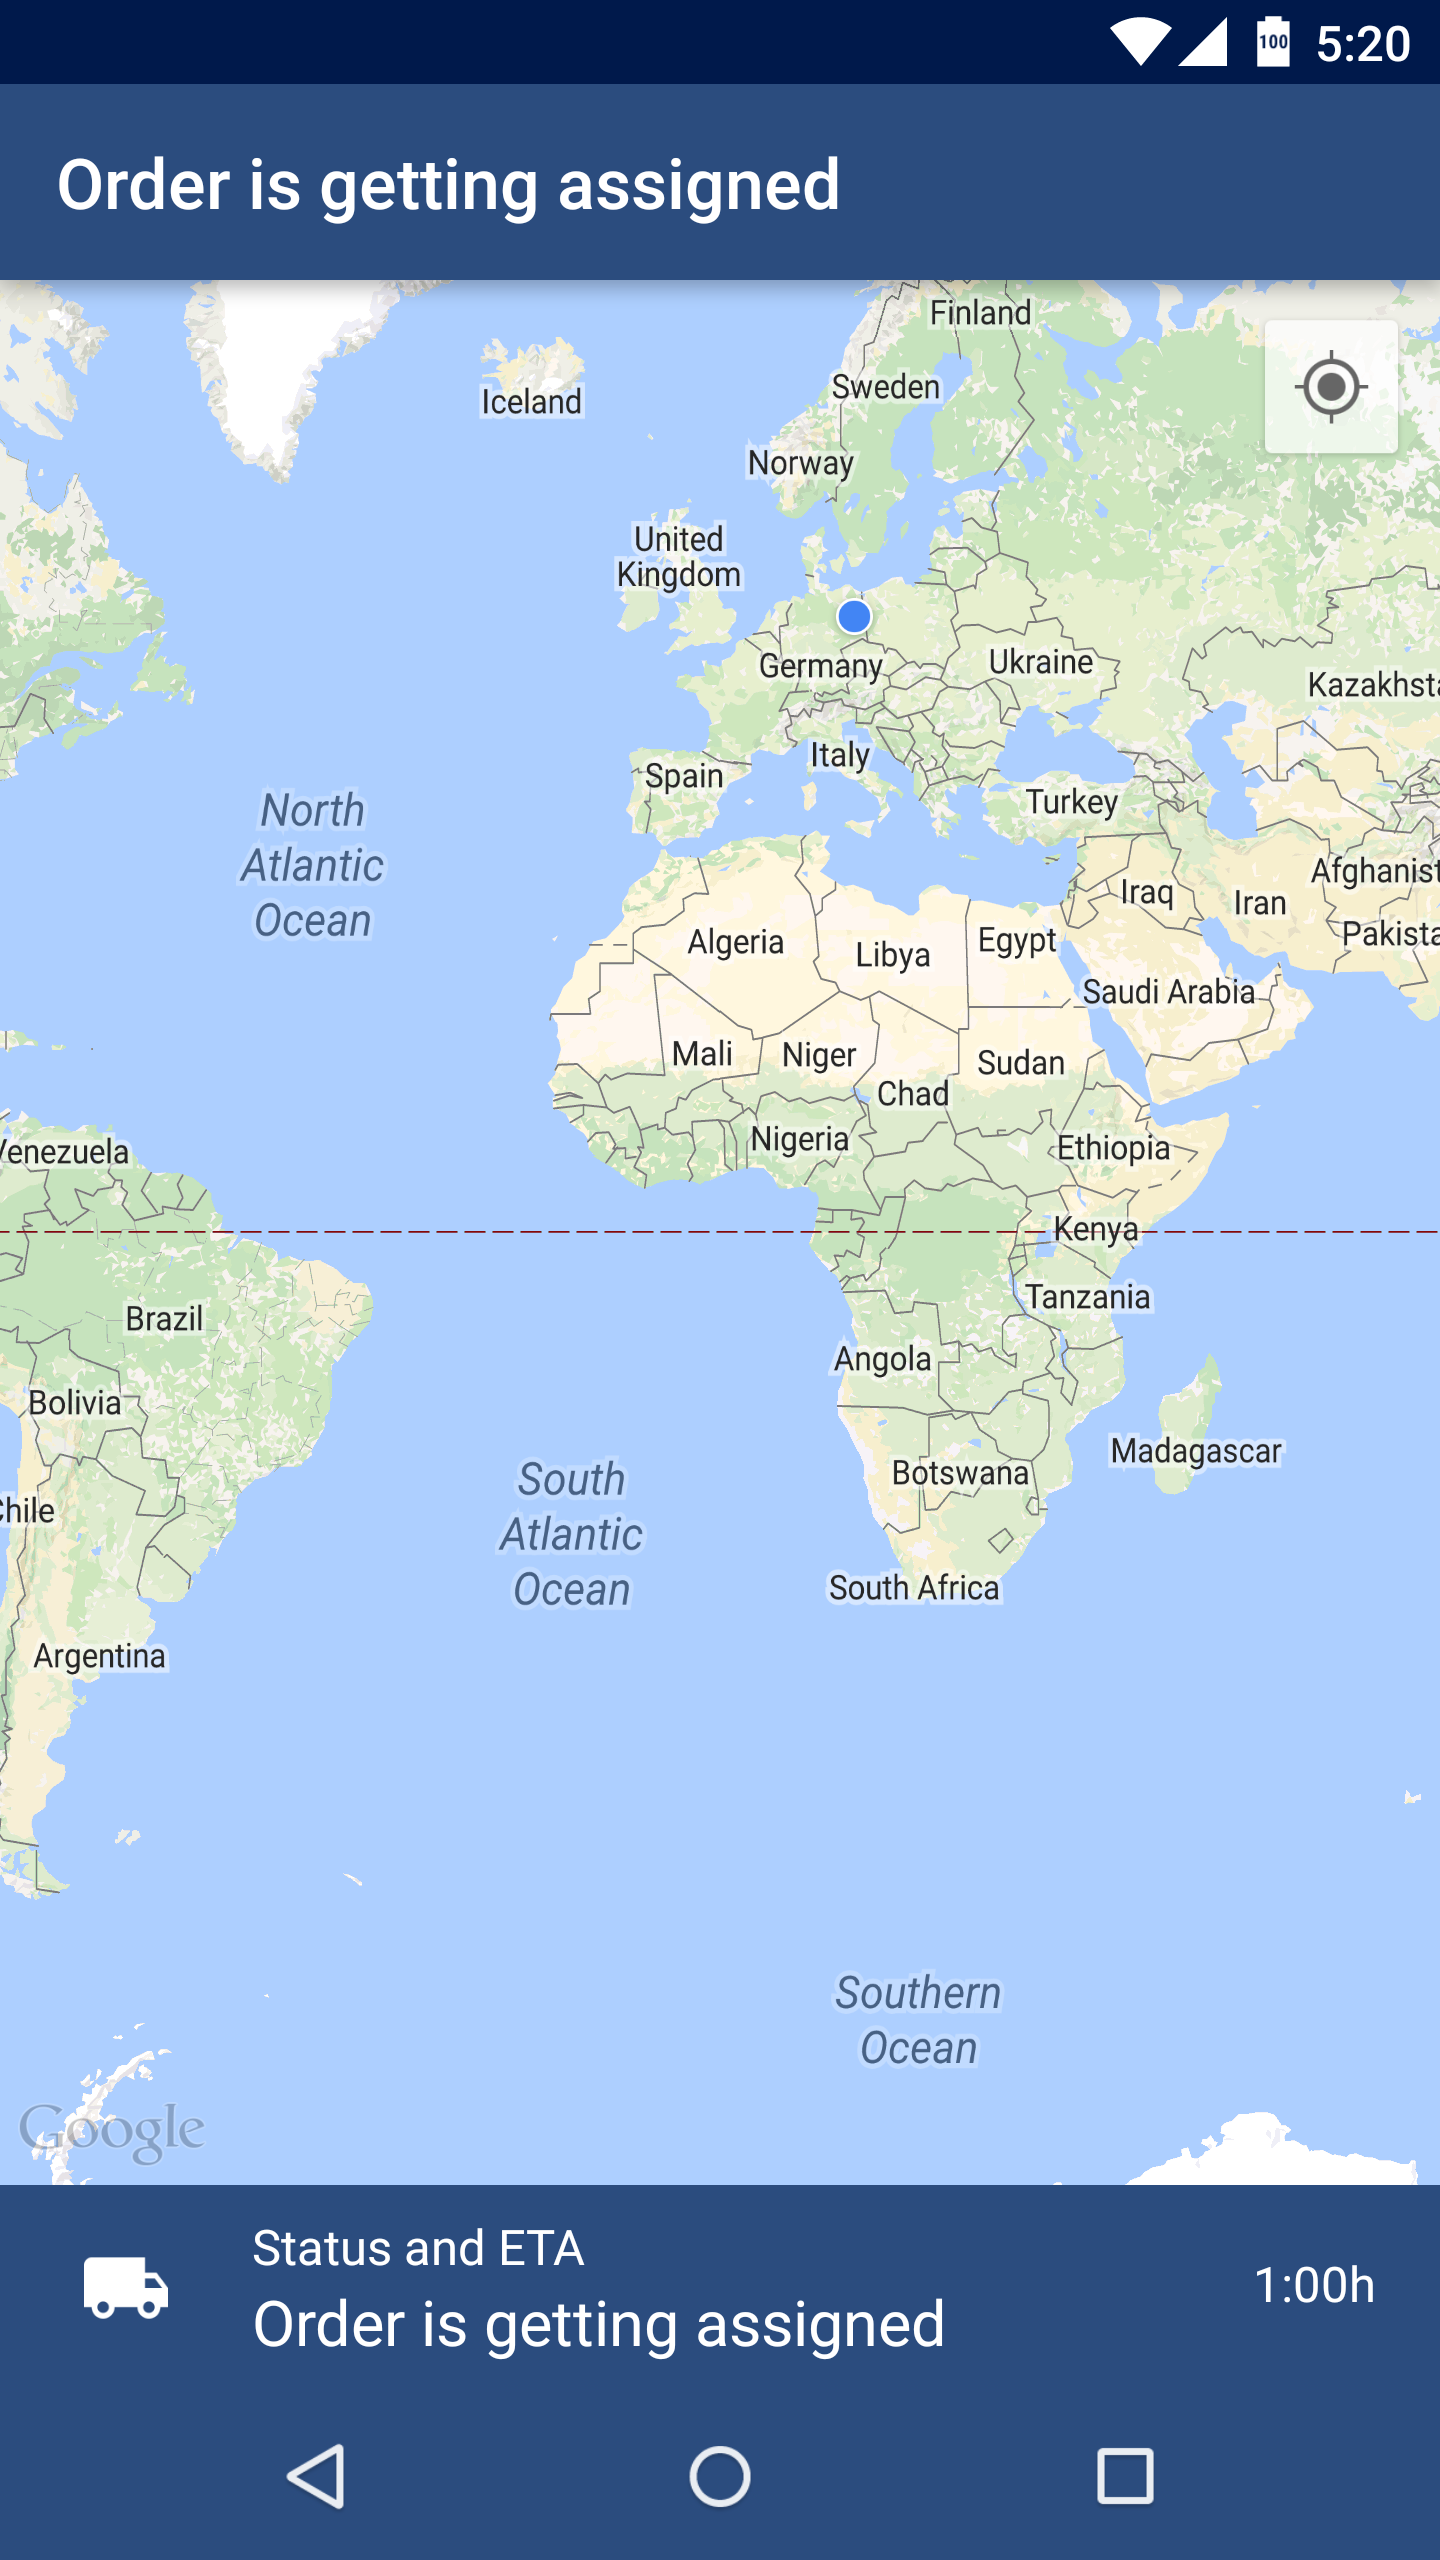
\includegraphics[width=.3\textwidth]{images/6_assign.png}\hfill
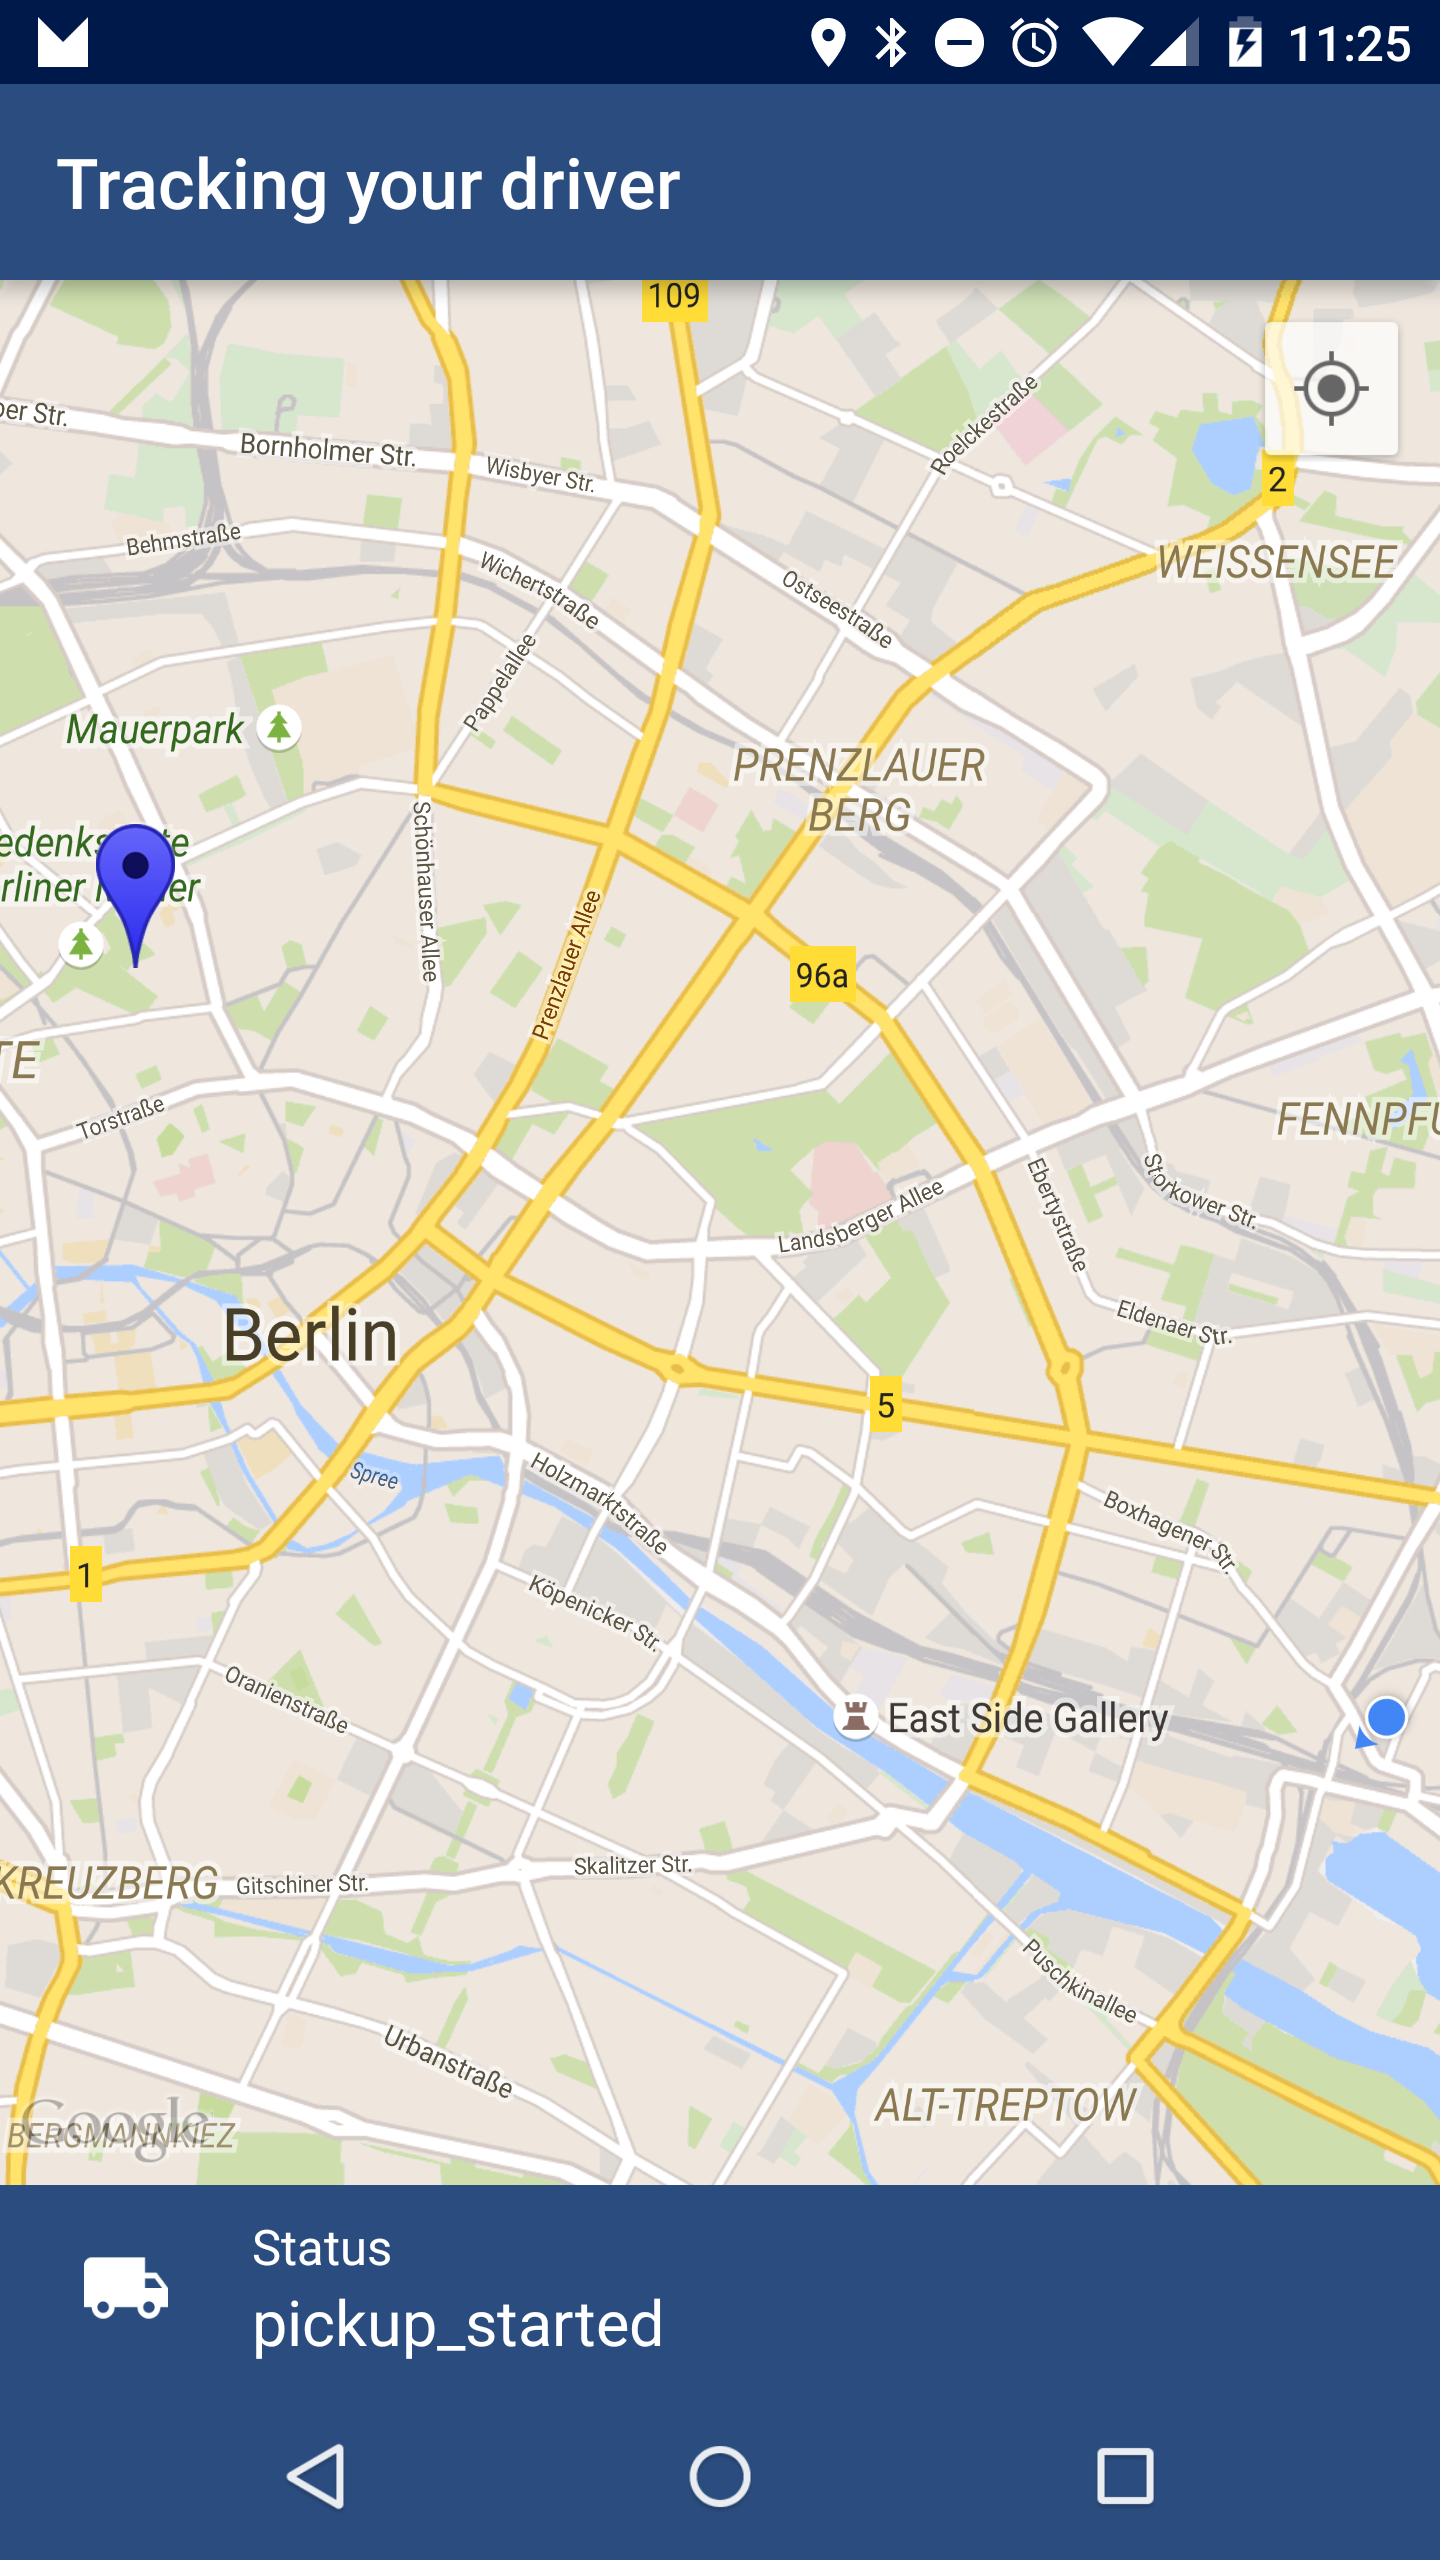
\includegraphics[width=.3\textwidth]{images/2_pickup_started.png}
\caption{The consumer application. Login on the left. Idle status in the middle. Pickup started on the right.}
\label{fig:consumer_application}

\end{figure}
The customer sees the different steps of the delivery process, namely \texttt{pickup\_ended}, when the driver has entered the restaurant, and \texttt{delivery\_started}, when the driver has left the restaurant with the meal (Figure \ref{fig:consumer_application2}, left and middle).
\begin{figure}[htp]

\centering
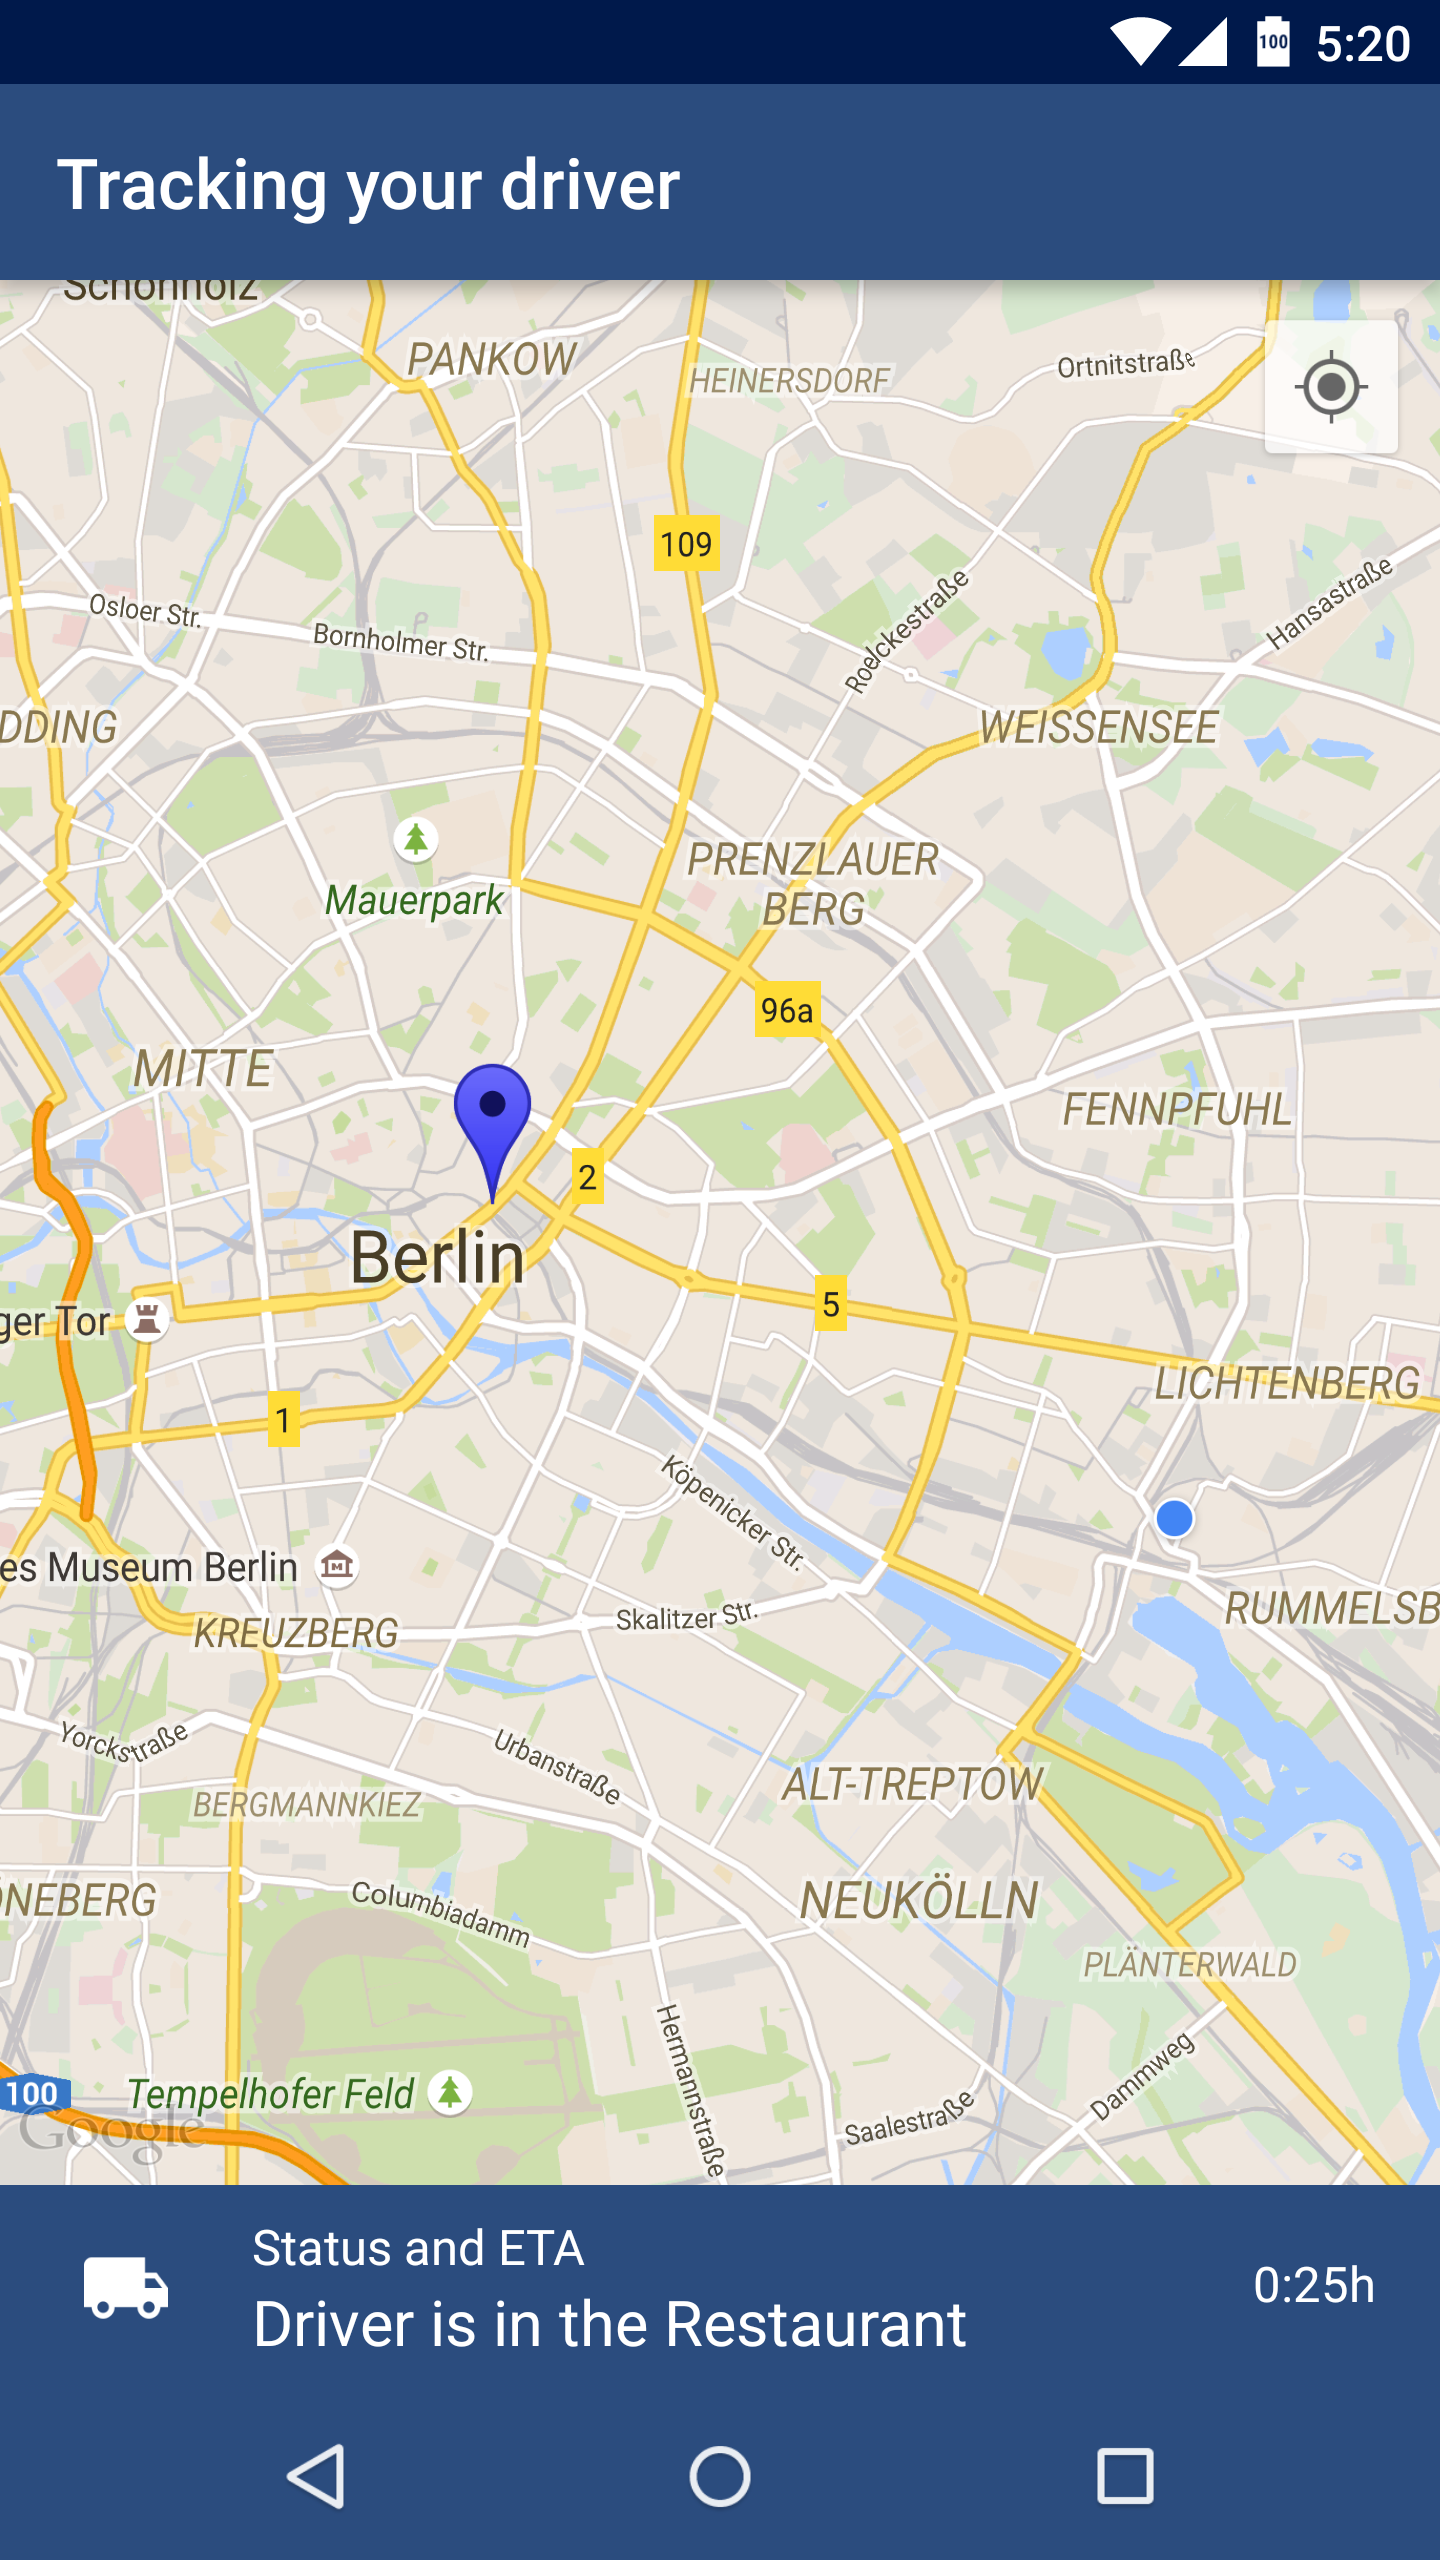
\includegraphics[width=.3\textwidth]{images/3_pickup_ended.png}\hfill
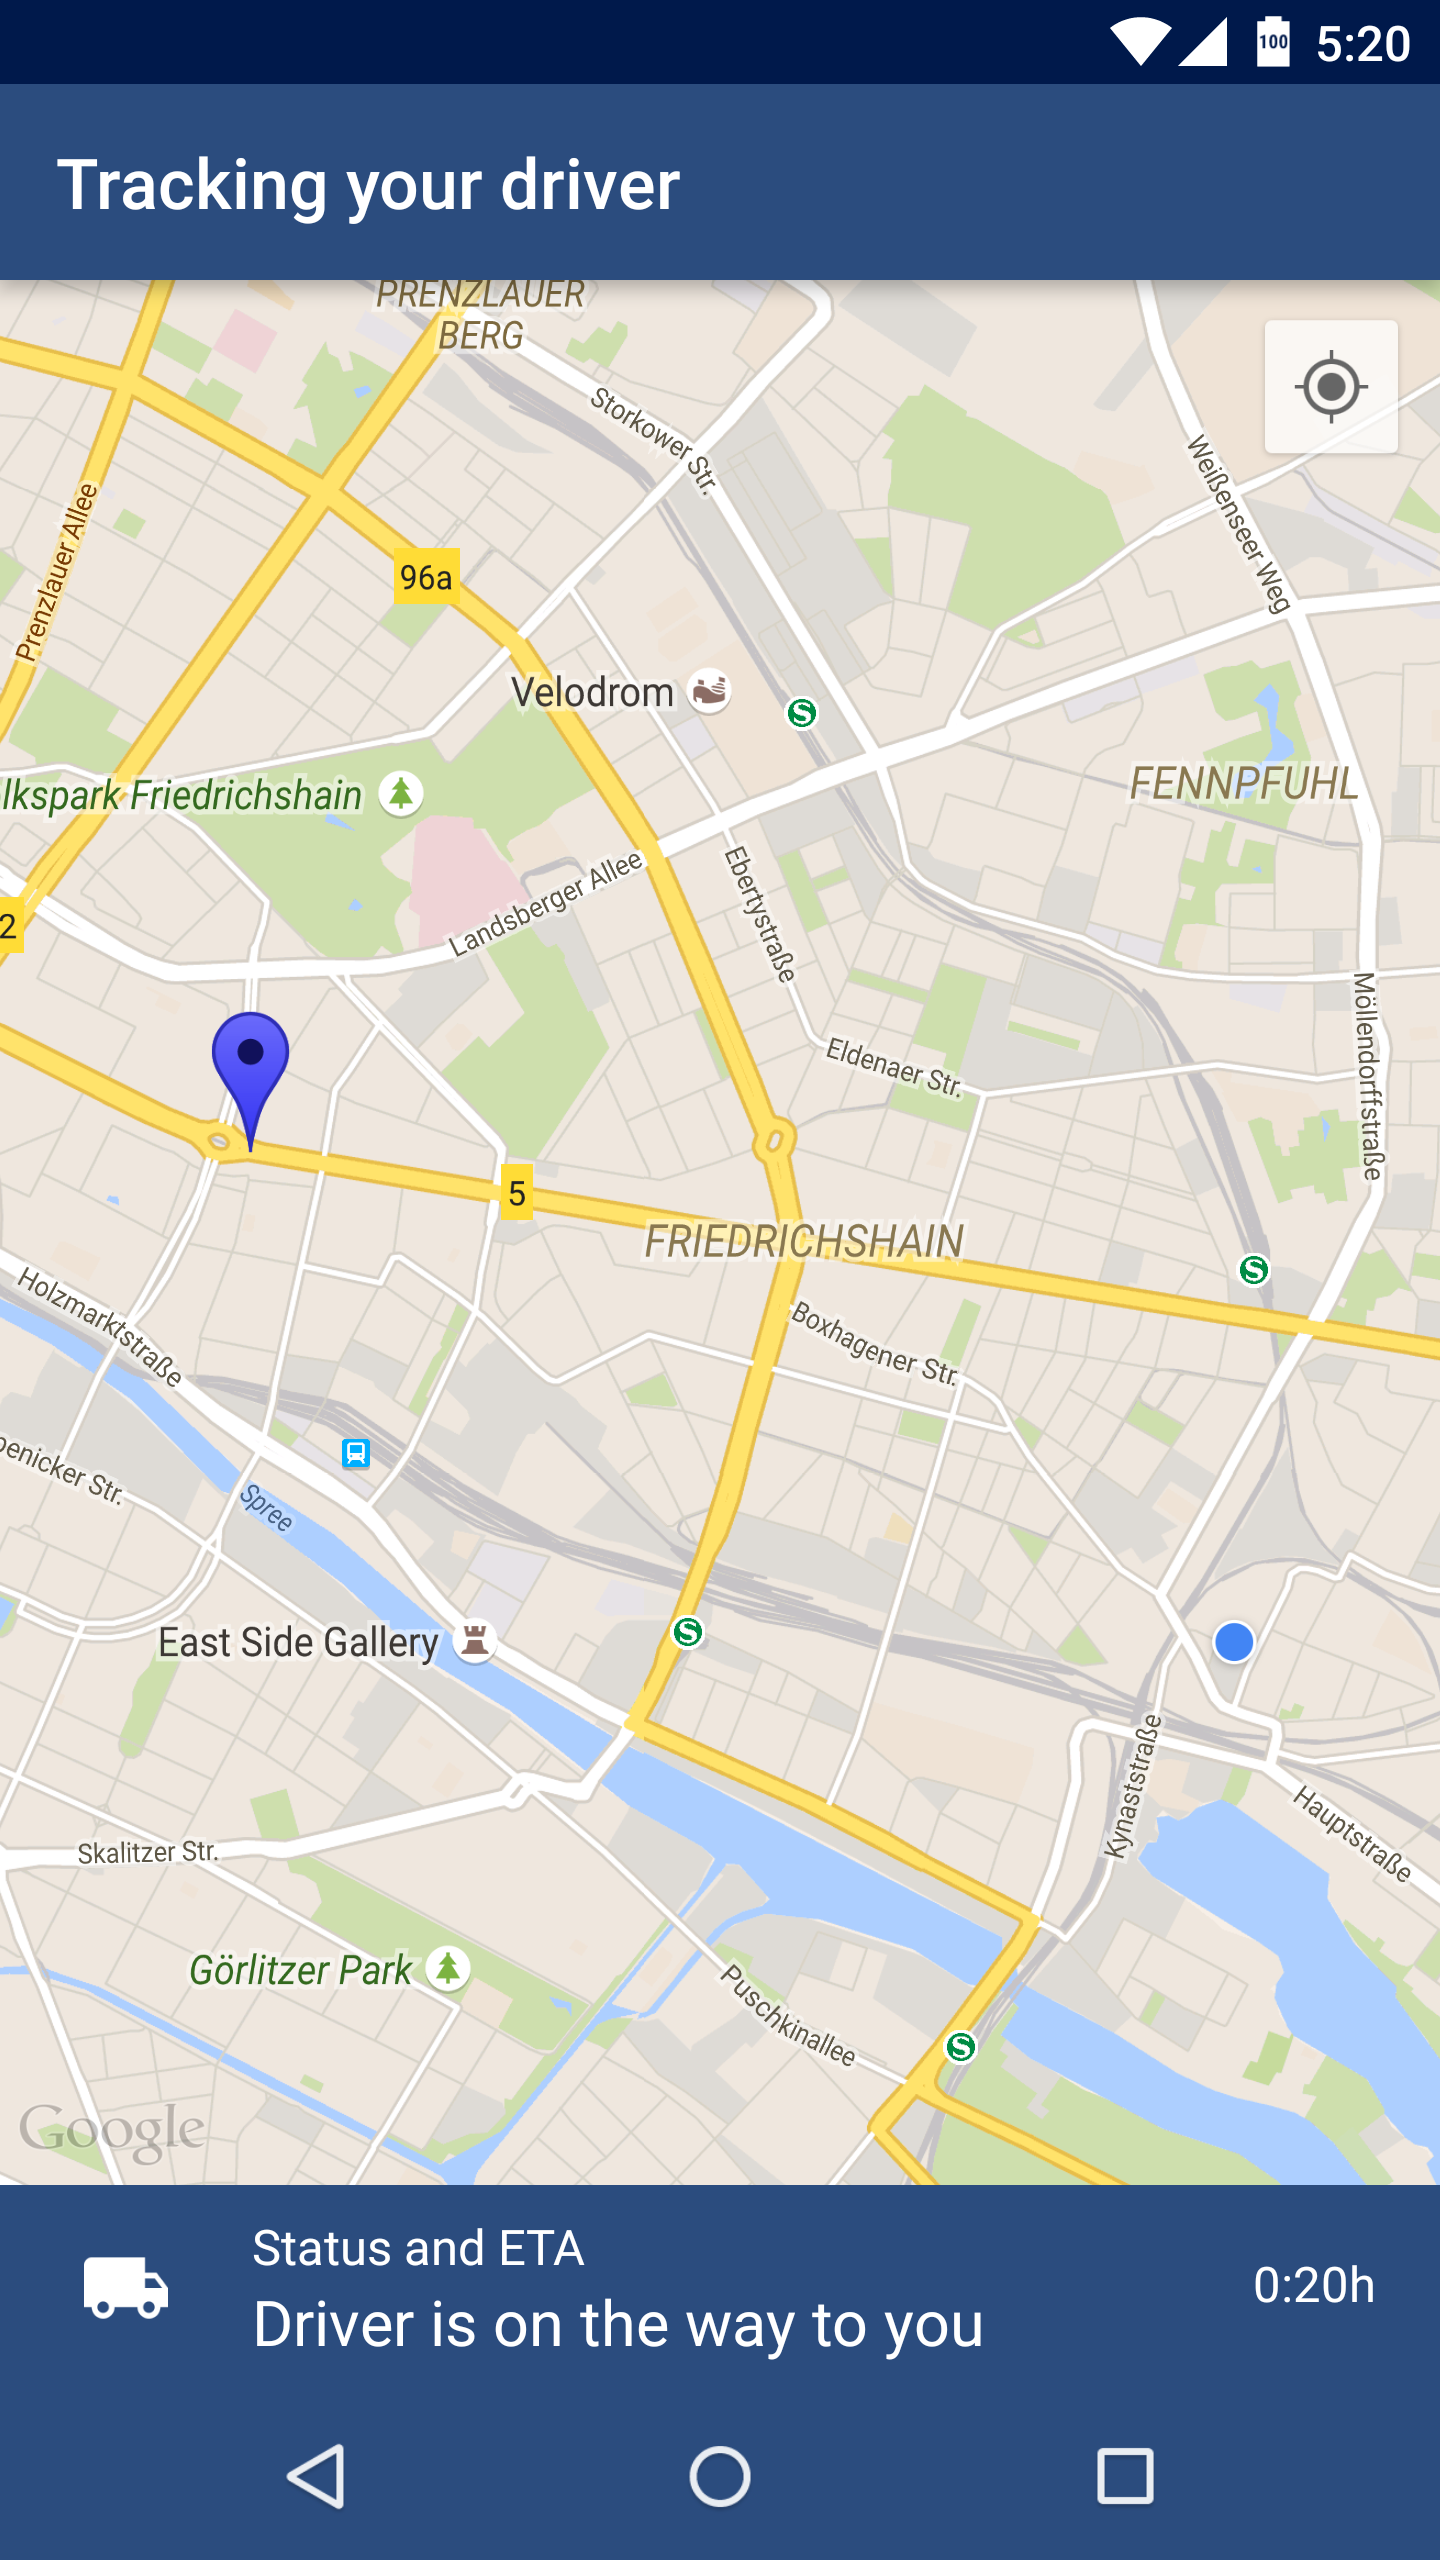
\includegraphics[width=.3\textwidth]{images/4_delivery_started.png}\hfill
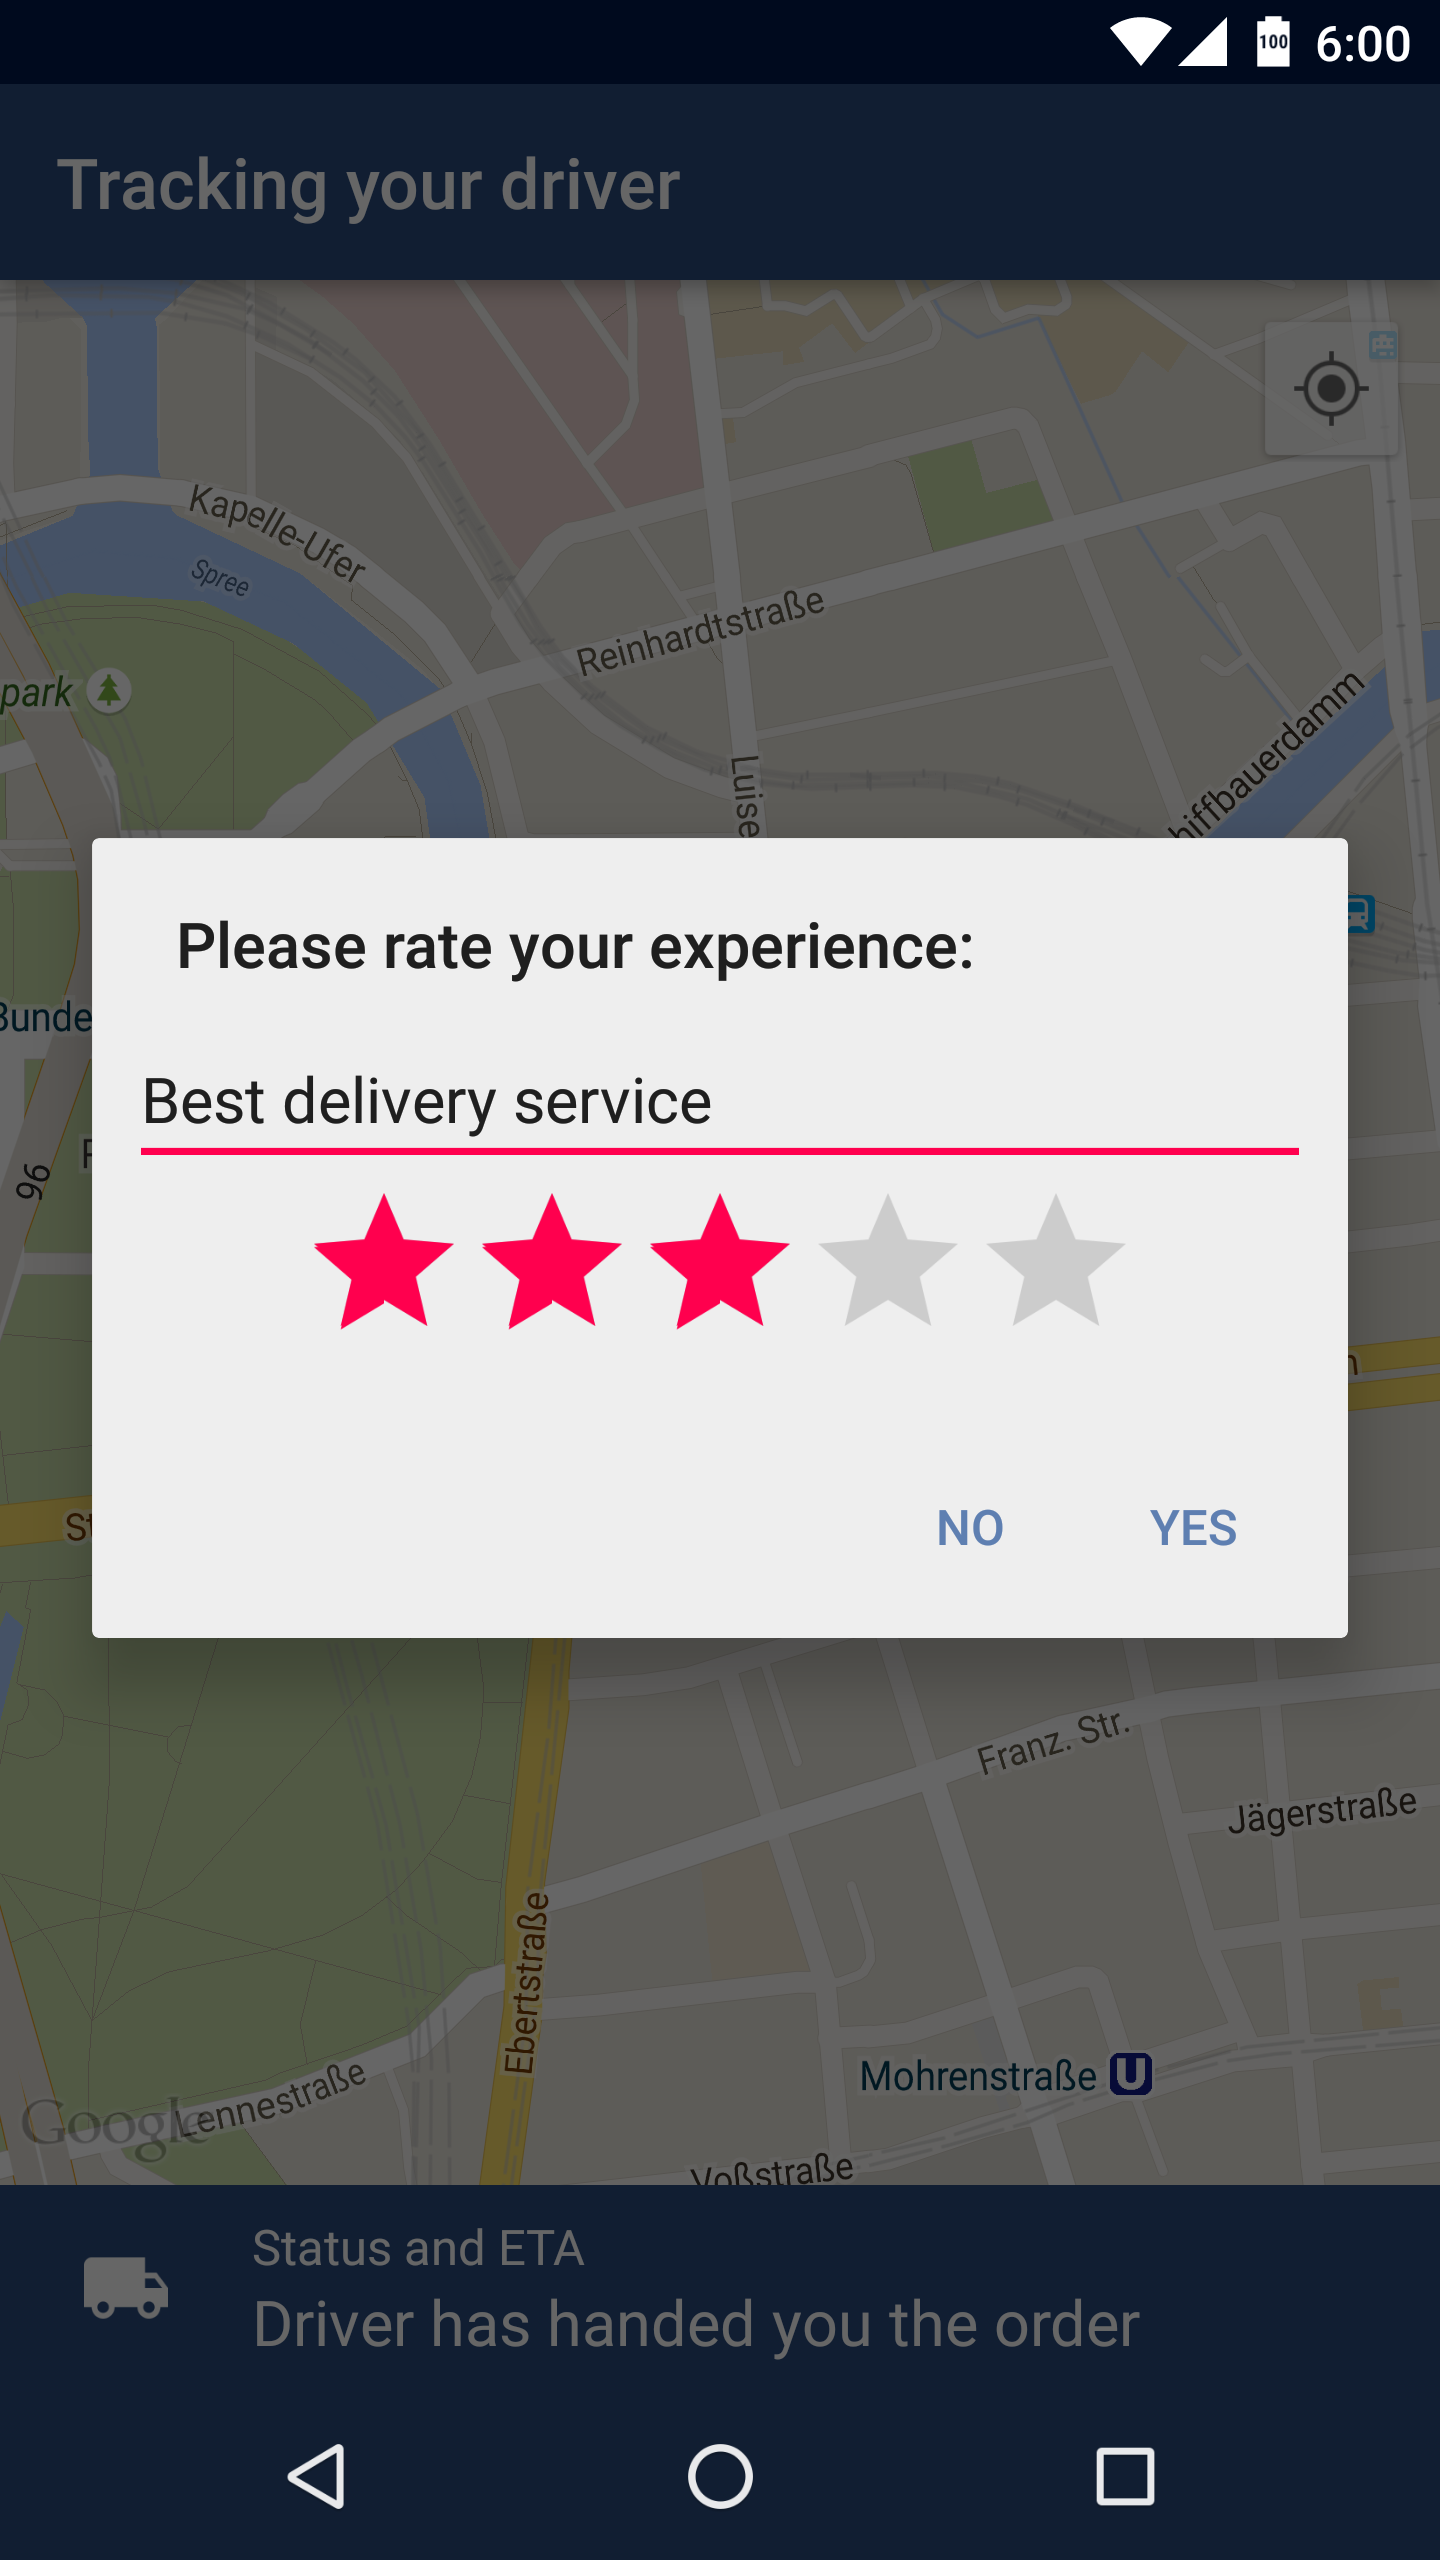
\includegraphics[width=.3\textwidth]{images/5_feedback.png}
\caption{The graphical user interface of the consumer application. When the driver is at the restaurant, when the driver has left the restaurant and when the driver has finished the delivery.}
\label{fig:consumer_application2}

\end{figure}

As soon as the driver has completed the delivery by giving the order to the customer and checking it in his driver application, a feedback dialog opens in the customer application(Figure \ref{fig:consumer_application2}, right). In this popup the customer can rate his experience and support valuable feedback for VOLO in case something was not as she wished.\newline
After entering the feedback, the application is closed and the user is logged out from the application. The credentials of the user are now set to inactive on the server since there is nothing to track anymore.\newline
This way the customer tracking application provides an easy and comfortable way of tracking an order and giving feedback about the delivery.
\newpage
\section{Appendix Two: Code and Results}\label{section:Appendix Two: Code and Results}

The code and application will be send by email since they contain confidential material of VOLO UG.
